\documentclass[twocolumn,letterpaper]{soups-poster}
\pdfpagewidth=8.5truein
\pdfpageheight=11truein

\usepackage{pifont}
\newcommand{\xmark}{\ding{55}}
\usepackage{lmodern}

\newcommand{\etal}[0]{et{.}~al{.}}
\newcommand{\citep}[1]{\cite{#1}}

\usepackage{listings}
\lstset{%
  basicstyle=\ttfamily\footnotesize,
  keywordstyle=\ttfamily\slshape\footnotesize,
  stringstyle=\ttfamily\bfseries\footnotesize,
  columns=flexible,
  tabsize=2,
  showstringspaces=true,
  %numbers=left,
  numberstyle=\tiny\ttfamily\color{Gray},
  commentstyle=\ttfamily\color{Gray}
}
\newcommand{\code}[2][]{\lstinline[#1]{#2}}
% Autoref line numebers
\providecommand*{\lstnumberautorefname}{line} 
% SecPAL
\lstdefinelanguage{apppal}{%
  morekeywords={says,if,where,False,True},%
  otherkeywords={=,0,inf,can-say,can-act-as},%
  morestring=[b]"%
}[keywords,comments,strings]
\lstset{language=apppal}

\usepackage{graphicx}
\renewcommand{\topfraction}{0.99} % be more aggressive about text around floats
\renewcommand{\floatpagefraction}{0.99}
\pagestyle{plain}

\begin{document}

\title{Using Authorization Logic to Capture User Policies in Mobile Ecosystems}
\numberofauthors{2}
\author{%
  \alignauthor{}
  Joseph Hallett\\
  \affaddr{University of Edinburgh}\\
  \email{joseph.hallett@sms.ed.ac.uk}
  \alignauthor{}
  David Aspinall\\
  \affaddr{University of Edinburgh}\\
  \email{david.aspinall@ed.ac.uk}
}
\date\today
\maketitle

\section{Introduction}

Mobile devices let users choose the software they want to run.
App stores offer a wide range of apps for users to pick from.
Users make the decision of which apps to use based on their own policies.
Sometimes this is based on what the store shows them first~\citep{Prata:2012in},
other times it is based on information about the app---ratings and the
permissions it requests~\citep{Kelley:2013kc}.

There is some evidence that users tend to fall into patterns when picking
apps~\citep{Sadeh:2014vq}.  By capturing these policies explicitly they can be
enforced more consistently by a machine, lessening the burden on users to decide
which apps they want.
Furthermore whilst some expert users could write their own policies formally, others
just want help.  By sharing policies users can gain the benefits of expert
written security policies without having to become experts themselves

\section{Policies and AppPAL}

\subsection{AppPAL}

To write policies we have used the AppPAL authorization logic.
AppPAL is a language, based on SecPAL~\citep{Becker:2006vh}, that can describe
what it means for an app to be installable. AppPAL requires all statements be
made by an explicit speaker, which enables rich delegation relationships to be
expressed in policies.
AppPAL is implemented as a Java library and runs on the Java and Dalvik virtual
machines.

Alice, a user, can state that a specific app is installable.
\begin{lstlisting}
"alice" says "com.rovio.angrybirds" isInstallable.
\end{lstlisting}
Alternately she can specify that an app is only installable if a set of
constraints (facts checkable by inspecting the app directly, or by static
analysis) are met.
She can also delegate parts of the decision to third parties, who in turn must
state facts about an app for it to be accepted.  An example might be a
that she will only install apps without the \texttt{LOCATION} permission
that meet her \emph{not-malware} policy (which she trusts McAfee to decide for
her).
\begin{lstlisting}
"alice" says App isInstallable
  if "not-malware-policy" isMetBy(App)
  where hasPermission(App, "LOCATION") = False.

"alice" says "mcafee" can-say 0
  "not-malware-policy" isMetBy(App).
\end{lstlisting}

\subsection{Policies}

Lin~\etal{} showed that users fall into four behaviour patterns when picking
apps~\citep{Sadeh:2014vq}.  Conservative users felt uncomfortable allowing an
app access to any personal data or functionality for any reason; unconcerned
users felt okay allowing access to any data for almost any reason.  Advanced
users were more picky, for example comfortable allowing apps access to location data for core
functionality but not for advertising purposes; whereas fence sitters (the
largest cluster) varied about what they found uncomfortable but were broadly
against collection of personal data for advertising purposes.

Using these behaviors as a start point we wrote the following AppPAL policies to
describe their behaviour, each of increasing strictness, each banning increasing
numbers of permissions.

\begin{tabular}{ r c c c c }\footnotesize
  & \rotatebox{90}{conservative} & \rotatebox{90}{advanced} & \rotatebox{90}{fencesitter} & \rotatebox{90}{unconcerned} \\
  \hline
  \lstinline{GET_ACCOUNTS}           & \xmark       & \xmark   & \xmark      & \xmark      \\
  \lstinline{ACCESS_FINE_LOCATION}   & \xmark       & \xmark   & \xmark      &             \\
  \lstinline{READ_CONTACT}           & \xmark       & \xmark   & \xmark      &             \\
  \lstinline{READ_PHONE_STATE}       & \xmark       & \xmark   &             &             \\
  \lstinline{SEND_SMS}               & \xmark       & \xmark   &             &             \\
  \lstinline{ACCESS_COARSE_LOCATION} & \xmark       &          &             &             \\
  \hline
\end{tabular}

% \begin{lstlisting}
% User says "unconcerned-policy" isMetBy(App)
%   if app isAnApp
%   where 
%     hasPermission(App, "GET_ACCOUNTS") = False.
%         
% User says "fencesitter-policy" isMetBy(App)
%   if "unconcerned-policy" isMetBy(App)
%   where 
%     hasPermission(App, "ACCESS_FINE_LOCATION") = False,
%     hasPermission(App, "READ_CONTACT") = False.
%
% User says "advanced-policy" isMetBy(App)
%   if "fencesitter-policy" isMetBy(App)
%   where 
%     hasPermission(App, "READ_PHONE_STATE") = False,
%     hasPermission(App, "SEND_SMS") = False,
%
% User says "conservative-policy" isMetBy(App)
%   if "advanced-policy" isMetBy(App)
%   where 
%     hasPermission(App, "ACCESS_COARSE_LOCATION") = False.
% \end{lstlisting}

McAfee classify malware into several categories. 
The \emph{malicious}, and \emph{trojan} categories describe traditional malware,
but there are other categories for PUS (potentially unwanted software).
Using AppPAL we can write policies to differentiate between these kinds of
malware.  This allows us to explore the difference between users with dangerous
apps installed and those who install merely unsavoury apps.
\begin{lstlisting}
User says McAfee can-say "malware" isKindOf(App).
McAfee says "trojan" can-act-as "malware".
McAfee says "pus" can-act-as "malware".
\end{lstlisting}

% We also add two additional policies.
% These policies use the categorization of apps (by the stores) to specify which
% policies based on how we might expect different kinds of apps to behave.
% A user might use app with in-app-purchases in general but decline
% games with them as they can be \emph{Cow Clickers}.
% \begin{lstlisting}
% User says "iap-policy" isMetBy(App)
%   if app isAnApp
%   where
%     hasGooglePlayCategory(App, "GAME") = False.
%
% User says "iap-policy" isMetBy(App)
%   if app isAnApp
%   where
%     hasGooglePlayCategory(App, "GAME") = True,
%     hasPermission(App, "com.android.vending.BILLING") = False.
% \end{lstlisting}

\section{Experiments}

\subsection{Aims}

We have two aims:to introduce AppPAL as a language for modelling and describing
app installation policies, and to measure the extent users currently enforce app
installation policies.

Our assumptions include:
\begin{itemize}
  \item Downloaded apps used for experiments are not the same version as those
    used by users; and may have different permissions. Permissions tend to grow
    in apps over time~\citep{Wei:2012id} (in part due to increased system
    permissions) so we might find the apps allowed are more permissive now than
    when the user installed them.

  \item We do not have the full user purchase history.
    We can only test policies on the apps we know about.
    Consequently a user may have apps installed that break the policy, but which
    we do not know.  This is a limitation of the Carat data set.
\end{itemize}

\subsection{Methodology}

We want to test how well these policies capture user behavior.
The Carat project~\citep{Oliner:2013ht} have a large, partially
anonymized\footnote{Users are replaced with incrementing numbers, apps with
hashes.},
database of app installations by users.  By calculating the hash of a package
name you can see which users installed which apps.

From an initial database of over 90,000 apps, and 55,000 users who on average
installed just under 90 apps each, we unmasked 4,300 apps (on average half the
  users installs).  Disregarding system apps (such as
\texttt{com.android.vending}) and very common apps such as Facebook, Dropbox,
Whatsapp, and Twitter we further reduced the set to an average of twenty apps
per user that they installed.

Using this data, and the apps themselves collected from the Google Play Store
and Android Observatory~\citep{Barrera:2012iba} we checked which apps satisfied
which AppPAL policies.  From here we created a table of whether a user's apps
satisfied a policy.

\subsection{Results}

\begin{figure}[!ht]
  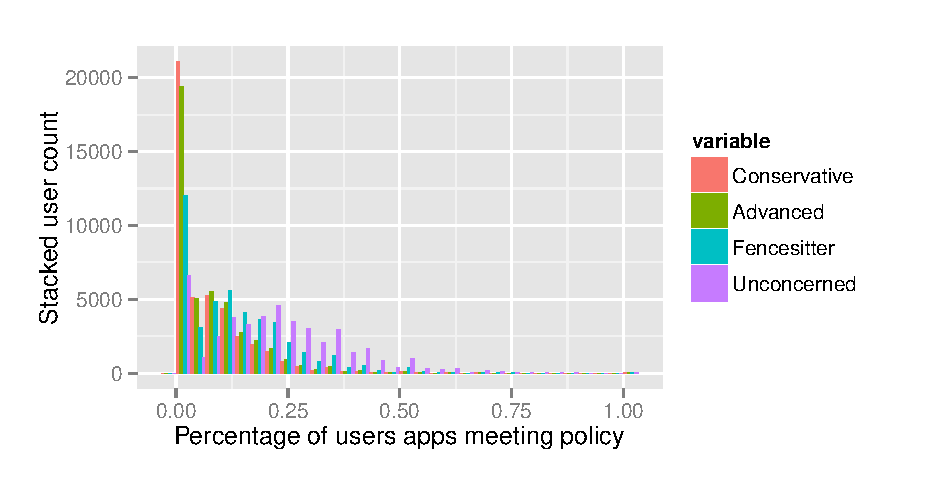
\includegraphics[width=\linewidth]{./tables/lin.eps}
  \caption{Adoption of policies modelling user behaviour.}
  \label{fig:lin}
\end{figure}

\begin{figure}[!ht]
  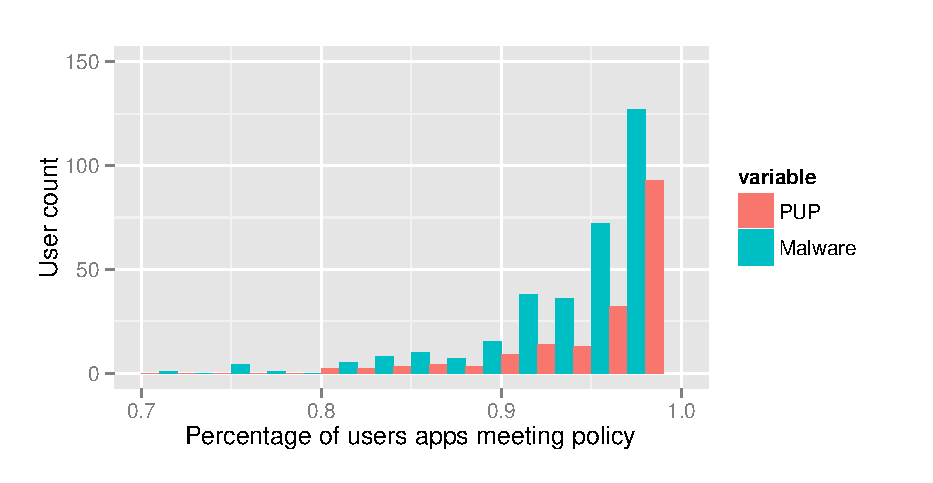
\includegraphics[width=\linewidth]{./tables/malware.eps}
  \caption{Adoption of policies for preventing PUS and malware.}
  \label{fig:malware}
\end{figure}

\section{Discussion}

In Figure~\ref{fig:lin} we can see that whilst the majority of users rarely
follow these policies there are a few users who do seem to be installing apps on
the basis of these policies most of the time.
With Figure~\ref{fig:malware} we see that most users do not install malware.
If we consider PUS separate from malware however, the number of users without
any PUS or malware is quartered.

AppPAL can, however, capture the differences in user policies and can be used to
filter apps on the basis of these policies.  Using AppPAL we have written
short policies describing user behaviour and been able to identify users
following them to varying degrees.

Next steps will involve a trial creating an app store for Android with AppPAL
built in.  This will allow us to trial the system with users
to begin exploring more complex policies to more accurately match their
behaviour and the explore what policies users want to have enforced.

\bibliographystyle{plain}
\bibliography{abstract}

\end{document}

